\documentclass[UTF8,AutoFakeBold,AutoFakeSlant,zihao=-4]{ctexart}
\usepackage[a4paper,left=3cm,right=2.4cm,top=2.6cm,bottom=2.38cm,includeheadfoot]{geometry}
\usepackage{fontspec}



\usepackage{xeCJK}
\setCJKmainfont{KaiTi}
\setmainfont{Times New Roman}

\setCJKfamilyfont{songti}{SimSun} %华文行楷  
\newcommand{\Mysongti}{\CJKfamily{songti}}  

\usepackage{graphicx}

%%
% 设置一级标题、二级标题格式
% 一级标题:小三,宋体,加粗,段前段后各半行
\ctexset{section={
		format={\raggedright \bfseries \Mysongti \zihao{-3}},
		beforeskip = 24bp plus 1ex minus .2ex,
		afterskip = 24bp plus .2ex,
		fixskip = true,
		name = {,.\quad}
	}
}
% 二级标题:小四,宋体,加粗,段前段后各半行
\ctexset{subsection={
		format = {\bfseries \Mysongti \raggedright \zihao{4}},
		beforeskip =24bp plus 1ex minus .2ex,
		afterskip = 24bp plus .2ex,
		fixskip = true,
	}
}


\begin{document}

	\title{Chapter13}
	\author{尹忠恩}
	\date{\today}
	\maketitle
	
	\newpage
	
	\section{实验01}
		\subsection{代码}
			
			\begin{verbatim}
				assume cs:code,ss:stack,ds:data
				
				data segment
				db 'welcome to masm!',0
				data ends
				
				stack segment
				db 128 dup(0)
				stack ends
				
				code segment
				start:
				mov ax,stack
				mov ss,ax
				mov sp,128
				
				call transfer
				call test_application
				
				mov ax,4c00h
				int 21h
				
				;=======================================
				test_application:
				push ax
				push bx
				push cx
				push dx
				push ds
				push es
				push si
				push di
				test_application_bg:
				mov dh,10;row
				mov dl,10;cul
				mov cl,2 ;color
				mov ax,data;ds:si
				mov ds,ax
				mov si,0
				int 7ch
				test_application_end:
				pop di
				pop si
				pop es
				pop ds
				pop dx
				pop cx
				pop bx
				pop ax
				ret
				;======================================= 
				transfer:
				push ax
				push bx
				push cx
				push dx
				push ds
				push es
				push si
				push di
				transfer_bg:
				;mov 7ch
				mov ax,cs
				mov ds,ax
				mov si,offset int_7ch
				
				mov ax,0
				mov es,ax
				mov di,200h
				
				mov cx,offset int_7ch_end - offset int_7ch
				
				cld
				rep movsb
				
				;set int table
				mov ax,0
				mov es,ax
				mov word ptr es:[7ch*4],200h
				mov word ptr es:[7ch*4+2],0
				transfer_end:
				pop di
				pop si
				pop es
				pop ds
				pop dx
				pop cx
				pop bx
				pop ax
				ret
				
				;===================================
				int_7ch:
				push ax
				push bx
				push cx
				push dx
				push ds
				push es
				push si
				push di
				int_7ch_bg:
				mov ax,0b800h
				mov es,ax
				mov di,0
				call get_row
				add di,ax
				call get_cul
				add di,ax
				
				
				
				s0:
				mov al,ds:[si]
				cmp al,0
				je end_0
				mov ah,cl
				mov es:[di],ax
				inc si
				inc di
				inc di
				jmp s0
				
				end_0:
				pop di
				pop si
				pop es
				pop ds
				pop dx
				pop cx
				pop bx
				pop ax
				iret
				
				get_row:
				mov al,160
				mul dh
				ret
				get_cul:
				mov al,2
				mul dl
				ret
				int_7ch_end:
				nop
				
				code ends
				end start
			\end{verbatim}
			
		\subsection{截图}
		
				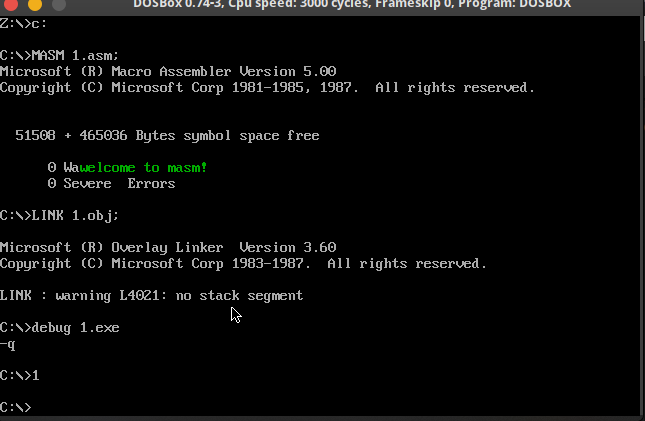
\includegraphics{chapter13.assets/001}
				
	\section{实验02}
		\subsection{代码}
			\begin{verbatim}
			assume cs:code,ss:stack,ds:data
			
			data segment
			db 'welcome to masm!',0
			data ends
			
			stack segment
			db 128 dup(0)
			stack ends
			
			code segment
			start:
			mov ax,stack
			mov ss,ax
			mov sp,128
			
			call transfer
			call test_application
			
			mov ax,4c00h
			int 21h
			
			;=======================================
			test_application:
			push ax
			push bx
			push cx
			push dx
			push ds
			push es
			push si
			push di
			test_application_bg:
			mov ax,0b800h
			mov es,ax
			mov di,160*12 ;position
			mov bx,offset s - offset test_application_end ;length
			mov cx,80 ;times
			s:
			mov byte ptr es:[di],'!'
			mov byte ptr es:[di+1],2
			add di,2
			int 7ch
			test_application_end:
			pop di
			pop si
			pop es
			pop ds
			pop dx
			pop cx
			pop bx
			pop ax
			ret
			;======================================= 
			transfer:
			push ax
			push bx
			push cx
			push dx
			push ds
			push es
			push si
			push di
			transfer_bg:
			;mov 7ch
			mov ax,cs
			mov ds,ax
			mov si,offset int_7ch
			
			mov ax,0
			mov es,ax
			mov di,200h
			
			mov cx,offset int_7ch_end - offset int_7ch
			
			cld
			rep movsb
			
			;set int table
			mov ax,0
			mov es,ax
			mov word ptr es:[7ch*4],200h
			mov word ptr es:[7ch*4+2],0
			transfer_end:
			pop di
			pop si
			pop es
			pop ds
			pop dx
			pop cx
			pop bx
			pop ax
			ret
			
			;===================================
			int_7ch:
			push ax
			push bx
			push dx
			push ds
			push es
			push si
			push di
			int_7ch_bg:
			
			push bp
			mov bp,sp
			dec cx
			jcxz end_7ch
			add [bp+2*8],bx
			
			
			end_7ch:
			
			pop bp
			
			pop di
			pop si
			pop es
			pop ds
			pop dx
			pop bx
			pop ax
			iret
			int_7ch_end:
			nop
			
			code ends
			end start
			\end{verbatim}
		\subsection{截图}
				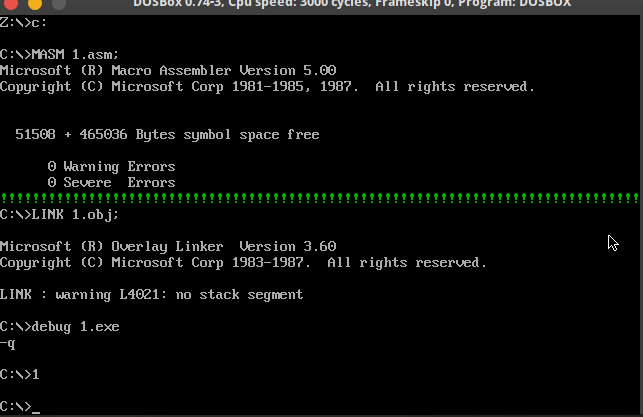
\includegraphics{chapter13.assets/002}
	\section{实验03}
		\subsection{代码}
			\begin{verbatim}
			assume cs:code
			
			code segment
			s1: db  'Good,better,best,','$'
			s2: db  'Never let it rest','$'
			s3: db  'Till good is better,','$'
			s4: db  'And better,best.','$'
			s:  dw  offset s1,offset s2,offset s3,offset s4
			row:    db 2,4,6,8
			
			start:
			
			call clear_screen
			call show
			
			mov ax,4c00h
			int 21h
			
			show:   
			push ax
			push bx
			push cx
			push dx
			push ds
			push es
			push si
			push di
			show_bg:
			mov ax,cs
			mov ds,ax
			mov bx,offset s
			mov si,offset row
			mov cx,4
			ok: mov bh,0
			mov dh,ds:[si]
			mov dl,0
			mov ah,2
			int 10h
			
			mov dx,ds:[bx]  
			mov ah,9
			int 21h
			
			inc si
			add bx,2
			
			loop ok
			show_end:
			pop di
			pop si
			pop es
			pop ds
			pop dx
			pop cx
			pop bx
			pop ax
			ret
			
			clear_screen:
			push ax
			push bx
			push cx
			push dx
			push ds
			push es
			push si
			push di
			clear_screen_bg:
			mov bx,0b800h
			mov es,bx
			
			mov bx,0
			mov dl,0
			mov dh,00000010b
			mov cx,2000
			
			clearScreen:	
			mov es:[bx],dx
			add bx,2
			
			loop clearScreen
			
			clear_screen_end:
			pop di
			pop si
			pop es
			pop ds
			pop dx
			pop cx
			pop bx
			pop ax
			ret
			
			
			code ends
			
			end start
			\end{verbatim}
		\subsection{截图}
				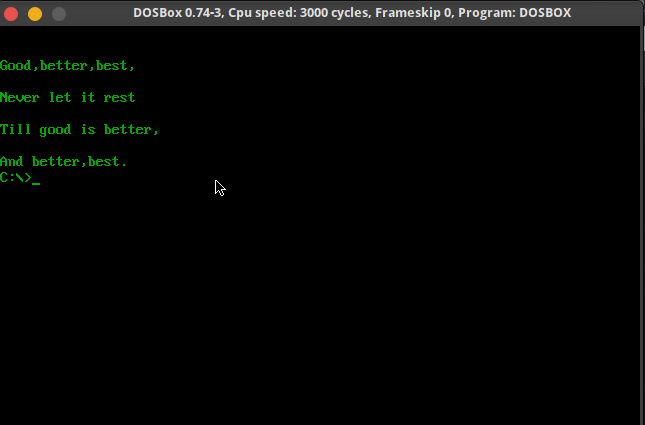
\includegraphics{chapter13.assets/003}
		
\end{document}